\documentclass[draftclsnofoot,onecolumn,letterpaper,10pt]{extras/IEEEtran}

%%%%%%%%%%%%%%%%%%%%%%%%%%%%%%%%%%%%%%%%%%%%%%%%%%%%%%%%%%%%%%%%%%%%%%%%%%%%%%%%
% Preamble
%% Note: Files in this directory are included in parent directory docs.
%% This means you need to source local files as `extras/file_name` instead of `file_name`.
%%%%%%%%%%%%%%%%%%%%%%%%%%%%%%%%%%%%%%%%%%%%%%%%%%%%%%%%%%%%%%%%%%%%%%%%%%%%%%%%
\usepackage{graphicx}                                        
\usepackage{amssymb}                                         
\usepackage{amsmath}                                         
\usepackage{amsthm}                                          

\usepackage{alltt}                                           
\usepackage{float}
\usepackage{color}
\usepackage{url}

%% \usepackage{balance}
%% \usepackage[TABBOTCAP, tight]{subfigure}
\usepackage{enumitem}
%% \usepackage{pstricks, pst-node}

\usepackage[margin=0.75in]{geometry}
\geometry{textheight=8.5in, textwidth=6in}

\graphicspath{ {imgs/} } 

\newcommand{\cred}[1]{{\color{red}#1}}
\newcommand{\cblue}[1]{{\color{blue}#1}}
\newcommand{\inlinecode}[1]{\texttt{#1}}

\usepackage{hyperref}
\usepackage{geometry}
\usepackage[english]{babel}
\usepackage{extras/titling}

\newcommand{\subtitle}[1]{%
  \posttitle{%
    \par\end{center}
    \begin{center}\large#1\end{center}
    \vskip0.5em}%
}

\usepackage{listings}
\usepackage{color}

\definecolor{mygreen}{rgb}{0,0.6,0}
\definecolor{mygray}{rgb}{0.5,0.5,0.5}
\definecolor{mymauve}{rgb}{0.58,0,0.82}

\lstset{ %
  backgroundcolor=\color{white},   % choose the background color; you must add \usepackage{color} or \usepackage{xcolor}
  basicstyle=\footnotesize\ttfamily,        % the size of the fonts that are used for the code
  breakatwhitespace=false,         % sets if automatic breaks should only happen at whitespace
  breaklines=true,                 % sets automatic line breaking
  captionpos=b,                    % sets the caption-position to bottom
  commentstyle=\color{mygreen},    % comment style
  deletekeywords={...},            % if you want to delete keywords from the given language
  escapeinside={\%*}{*)},          % if you want to add LaTeX within your code
  extendedchars=true,              % lets you use non-ASCII characters; for 8-bits encodings only, does not work with UTF-8
}


\title{High Performance XML/XSLT Transformation Server}
\subtitle{Client Requirements}
\author{
  \IEEEauthorblockN{Zixun Lu (luzi),}
  \IEEEauthorblockN{Shuai Peng (pengs),}
  \IEEEauthorblockN{Elijah Voigt (voigte)}
  \IEEEauthorblockA{\\CS 461 | CS Senior Capstone \\ Fall 2016}
}
\date{\today}

%%%%%%%%%%%%%%%%%%%%%%%%%%%%%%%%%%%%%%%%%%%%%%%%%%%%%%%%%%%%%%%%%%%%%%%%%%%%%%%%
% Document
%%%%%%%%%%%%%%%%%%%%%%%%%%%%%%%%%%%%%%%%%%%%%%%%%%%%%%%%%%%%%%%%%%%%%%%%%%%%%%%%
\begin{document}

%%%%%%%%%%%%%%%%%%%%%%%%%%%%%%%%%%%%%%%%%%%%%%%%%%%%%%%%%%%%%%%%%%%%%%%%%%%%%%%%
% Title Page
%%%%%%%%%%%%%%%%%%%%%%%%%%%%%%%%%%%%%%%%%%%%%%%%%%%%%%%%%%%%%%%%%%%%%%%%%%%%%%%%
\maketitle
\begin{abstract}
  (abstract text)

\end{abstract}

\clearpage

%%%%%%%%%%%%%%%%%%%%%%%%%%%%%%%%%%%%%%%%%%%%%%%%%%%%%%%%%%%%%%%%%%%%%%%%%%%%%%%%
% Document Content
%
% NB: You are required to have your client physically sign the document, print it out, and submit it to me in hardcopy as well as ensuring there is an unsigned digital copy.
%Yes, I want both.
%
% A Requirements Document outlines your project so that (1) you know what you are doing, and (2) your Client knows what they are getting.
%It is always a good idea to get that fixed ahead of time.
%
% You will be creating a team name for this project, and including it in your requirements document.
%Remember, the client will be approving this document, so pick a name that is fun and makes you happy, but is also at least vaguely professional.
% I like to think of this as an exercise in naming a company -- in other words, if you were to productize this project and sell it, this team name would be the name of your company.
%
% You will be making use of IEEE Std 830-1998 as the formatting guidelines for this document.
% You will also be required to make use of LaTeX for this document.
% See the course website for recorded lectures and learning material to help if you have not used LaTeX before.
%
% While the IEEE 830 format may be new, this should significantly draw on knowledge learned in the prerequisite Software Engineering I course you've taken.
% If unsure, please discuss this with your TA or myself prior to submission or sending to the client.
%
% This is very much the "what" document describing your project.
% The different requirements should be at the individual task level.
% You can do this as user stories (for something like a kanban board), or you can do it as something more at the functional level.
% Either way, make sure that you do these at a sufficient level of granularity such that you can mark them as complete as you go.
%
% You will be creating a Gantt Chart for this.
% How you do this is up to you
%%%%%%%%%%%%%%%%%%%%%%%%%%%%%%%%%%%%%%%%%%%%%%%%%%%%%%%%%%%%%%%%%%%%%%%%%%%%%%%%

\section{Introduction}

\subsection{Purpose}
The purpose of this document is to present a detailed description of high performance XML/XSLT transformation server.
This document is intended for people who maintain server and the developers of the system. 
%%%%%%%%%%%%%%%%%%%%%%%%%%%%%%%%%%%%%%%%%%%%%%%%%%%%%%%%%%%%%%%%%%%%%%%%%%%%%%%%
% Delineate the purpose of the SRS
% Specify the intended audience of the SRS
%%%%%%%%%%%%%%%%%%%%%%%%%%%%%%%%%%%%%%%%%%%%%%%%%%%%%%%%%%%%%%%%%%%%%%%%%%%%%%%%

\subsection{Scope}
This software system will create a high performance XML/XSLT transformation server that can perform repetitive document transformations in a high-volume environment. 
XSLT is used to convert an XML document to another XML document, or other types of documents that can be recognized by the browser, such as HTML and XHTML. 
In normal, XSLT accomplishes this by converting each XML element to an (X)HTML element. With XSLT, you can add or remove elements and attributes from or to the output file. 
You can also rearrange elements, perform tests, and decide which elements to hide or display. 
%%%%%%%%%%%%%%%%%%%%%%%%%%%%%%%%%%%%%%%%%%%%%%%%%%%%%%%%%%%%%%%%%%%%%%%%%%%%%%%%
% 1. Identify the software product(s) to be produced by name (e.g., Host DBMS, Report Generator, etc.);
% 2. Explain what the software product(s) will, and, if necessary, will not do;
% 3. Describe the application of the software being specified, including relevant benefits, objectives, and goals;
% 4. Be consistent with similar statements in higher-level specifications (e.g., the system requirements specification), if they exist.
%%%%%%%%%%%%%%%%%%%%%%%%%%%%%%%%%%%%%%%%%%%%%%%%%%%%%%%%%%%%%%%%%%%%%%%%%%%%%%%%

\subsection{Definitions, acronyms, and abbreviations}
XML is a simple and standard way of exchanging raw data between computer programs.
It is not only easy to be written and read but also solve the application of information exchange between systems. 
There are two basic needs:
(1) Separate the data from the representation
(2) Transfer data between different applications
In order to make the data easy for people to read and understand, we need to display information or pint out. For example, the data into an HTML file, a PDF file, or even a sound. Similarly, in order to adapt the data to different applications, a data format is converted to another data format, such as the demand format may be a text file, a SQL statement and an HTTP message. XSLT is used to achieve this conversion function of the language. XML is converted to HTML, XSLT is the most important function. 
XSLT: Extensible Stylesheet Language Transformations
XML: eXtensible Markup Language


%%%%%%%%%%%%%%%%%%%%%%%%%%%%%%%%%%%%%%%%%%%%%%%%%%%%%%%%%%%%%%%%%%%%%%%%%%%%%%%%
% Provide the definitions of all terms, acronyms, and abbreviations required to properly interpret the SRS.
% This information may be provided by reference to one or more appendixes in the SRS or by reference to other documents.
%%%%%%%%%%%%%%%%%%%%%%%%%%%%%%%%%%%%%%%%%%%%%%%%%%%%%%%%%%%%%%%%%%%%%%%%%%%%%%%%

\subsection{References}
IEEE. IEEE Std 830-1998 IEEE Recommended Practice for Software Requirements Specifications. IEEE Computer Society, 1998.

%%%%%%%%%%%%%%%%%%%%%%%%%%%%%%%%%%%%%%%%%%%%%%%%%%%%%%%%%%%%%%%%%%%%%%%%%%%%%%%%
% 1. Provide a complete list of all documents referenced elsewhere in the SRS;
% 2. Identify each document by title, report number (if applicable), date, and publishing organization;
% 3. Specify the sources from which the references can be obtained.
% 4. This information may be provided by reference to an appendix or to another document.
%%%%%%%%%%%%%%%%%%%%%%%%%%%%%%%%%%%%%%%%%%%%%%%%%%%%%%%%%%%%%%%%%%%%%%%%%%%%%%%%

\cite{xalan}
\cite{xerces}
\cite{icu}

\bibliographystyle{plain}
\bibliography{sections/references}

\subsection{Overview}
The next chapter, the Overall Description Section, of this document gives an overview of the
functionality of the product. It describes the informal requirements and is used to establish a context for the technical requirements specification in the next chapter.
The third chapter, Requirements Specification section, of this document is written primarily for the developers and describes in technical terms the details of the functionality of the product.
Both sections of the document describe the same software product in its entirety, but are intended for different audiences and thus use different language.


%%%%%%%%%%%%%%%%%%%%%%%%%%%%%%%%%%%%%%%%%%%%%%%%%%%%%%%%%%%%%%%%%%%%%%%%%%%%%%%%
% Describe what the rest of the SRS contains;
% Explain how the SRS is organized
%%%%%%%%%%%%%%%%%%%%%%%%%%%%%%%%%%%%%%%%%%%%%%%%%%%%%%%%%%%%%%%%%%%%%%%%%%%%%%%%


\section{Overall description}

%%%%%%%%%%%%%%%%%%%%%%%%%%%%%%%%%%%%%%%%%%%%%%%%%%%%%%%%%%%%%%%%%%%%%%%%%%%%%%%%
% This section of the SRS should describe the general factors that affect the product and its requirements.
% This section does not state specific requirements.
% Instead, it provides a background for those requirements, which are defined in detail in Section 3 of the SRS, and makes them easier to understand.
%%%%%%%%%%%%%%%%%%%%%%%%%%%%%%%%%%%%%%%%%%%%%%%%%%%%%%%%%%%%%%%%%%%%%%%%%%%%%%%%

The following sections of this document outline the factors that affect the creation of XZES40-Transformer at a high-level.

\subsection{Product perspective}
%%%%%%%%%%%%%%%%%%%%%%%%%%%%%%%%%%%%%%%%%%%%%%%%%%%%%%%%%%%%%%%%%%%%%%%%%%%%%%%%
% This subsection of the SRS should put the product into perspective with other related products.
% If the product is independent and totally self-contained, it should be so stated here.
% If the SRS defines a product that is a component of a larger system, as frequently occurs,
% then this subsection should relate the requirements of that larger system to functionality of the software and should identify interfaces between that system and the software.
% A block diagram showing the major components of the larger system, interconnections, and external interfaces can be helpful.
% This subsection should also describe how the software operates inside various constraints.
% For example, these constraints could include
% 1. System interfaces;
% 2. User interfaces;
% 3. Hardware interfaces;
% 4. Software interfaces;
% 5. Communications interfaces;
% 6. Memory;
% 7. Operations;
% 8. Site adaptation requirements.
%%%%%%%%%%%%%%%%%%%%%%%%%%%%%%%%%%%%%%%%%%%%%%%%%%%%%%%%%%%%%%%%%%%%%%%%%%%%%%%%

\subsubsection{System interfaces}
%%%%%%%%%%%%%%%%%%%%%%%%%%%%%%%%%%%%%%%%%%%%%%%%%%%%%%%%%%%%%%%%%%%%%%%%%%%%%%%%
% This should list each system interface and identify the functionality of the software to accomplish the system requirement and the interface description to match the system.
%%%%%%%%%%%%%%%%%%%%%%%%%%%%%%%%%%%%%%%%%%%%%%%%%%%%%%%%%%%%%%%%%%%%%%%%%%%%%%%%

XZES40-Transformer application will interface with the outside world through an Apache CGI script.
This script will wrap our application by passing \inlinecode{POST} requests to the application URL endpoint through to our application.
Our program will complete the request and pass the transformed document back to the user via the CGI script.

The XZES40-Transformer CGI wrapper script will receive a transformation request in the form of a \inlinecode{HTTP POST} request from a user and respond with the transformed file and an \textbf{OK} status.
If an error occurs it will respond with a \textbf{SERVER ERROR} response and no file.

% \begin{enumerate}
%   \item Data base
%   \item User and manager
%   \item XML servers
% \end{enumerate}
%
% Our server has 3 layer of actor, first layer is user part, such as reader and manager.
% Second layer is XML servers, which contain XML parse and other XML transformation part.
% Third layer is our database where we store our data.
% User can connect to webpage and send request to XML servers,and then XML servers will search from database and query data out, after that XML server can compile to Unicode type file and give back to user.

\subsubsection{User interfaces}
%%%%%%%%%%%%%%%%%%%%%%%%%%%%%%%%%%%%%%%%%%%%%%%%%%%%%%%%%%%%%%%%%%%%%%%%%%%%%%%%
% This should specify 
% 1. The logical characteristics of each interface between the software product and its users.
%    This includes those configuration characteristics (e.g., required screen formats, page or window layouts, 
%    content of any reports or menus, or availability of programmable function keys) necessary to accomplish the software requirements.
% 2. All the aspects of optimizing the interface with the person who must use the system.
%    This may simply comprise a list of do's and don'ts on how the system will appear to the user.
%    One example may be a requirement for the option of long or short error messages.
%    Like all others, these requirements should be verifiable, e.g., “a clerk typist grade 4 can do function X in Z min after 1 h of training” rather than “a typist can do function X.” (This may also be specified in the Software System Attributes under a section titled Ease of Use.)
%%%%%%%%%%%%%%%%%%%%%%%%%%%%%%%%%%%%%%%%%%%%%%%%%%%%%%%%%%%%%%%%%%%%%%%%%%%%%%%%

XZES40 will have two user interfaces which will access it's functionality over the internet.

\begin{itemize}
    \item A Website to access XZES40-Transformer via a web-browser.
    \item A CLI to access XZES40-Transformer via a terminal interface.
\end{itemize}
% Our application requires at least 800x600 resolution and 256 color monitor, and standard keyboard, and mouse is option.
% Managers can control database in their experience after see the GUI of transfer management application.
% User just need click webpage request, and other things is working behind the webpage.

\subsubsection{Hardware interfaces}
%%%%%%%%%%%%%%%%%%%%%%%%%%%%%%%%%%%%%%%%%%%%%%%%%%%%%%%%%%%%%%%%%%%%%%%%%%%%%%%%
% This should specify the logical characteristics of each interface between the software product and the hardware components of the system.
% This includes configuration characteristics (number of ports, instruction sets, etc.).
% It also covers such matters as what devices are to be supported, how they are to be supported, and protocols.
% For example, terminal support may specify full-screen support as opposed to line-by-line support.
%%%%%%%%%%%%%%%%%%%%%%%%%%%%%%%%%%%%%%%%%%%%%%%%%%%%%%%%%%%%%%%%%%%%%%%%%%%%%%%%

XZES-Transformer will be targeted to run on an x86-64 CPU architecture server.
Any computer with a browser will be able to access the web-interface.

XZES40-Transformer will not have any direct physical interfaces as it is meant to be interacted with over \inlinecode{HTTP/HTTPS}.

% We will support windows, Unix based operation  system, iOS and android.
% We will create API for our application, so we can easy to move application to any platform.
% GUI is required rather than line by line terminal control.

\subsubsection{Software interfaces}
%%%%%%%%%%%%%%%%%%%%%%%%%%%%%%%%%%%%%%%%%%%%%%%%%%%%%%%%%%%%%%%%%%%%%%%%%%%%%%%%
% This should specify the use of other required software products (e.g., a data management system, an operating system, or a mathematical package),
% and interfaces with other application systems (e.g., the linkage between an accounts receivable system and a general ledger system).
% For each required software product, the following should be provided:
% - Name;
% - Mnemonic;
% - Specification number;
% - Version number;
% - Source.
% For each interface, the following should be provided:
% - Discussion of the purpose of the interfacing software as related to this software product.
% - Definition of the interface in terms of message content and format.
%   It is not necessary to detail any well-documented interface, but a reference to the document defining the interface is required.
%%%%%%%%%%%%%%%%%%%%%%%%%%%%%%%%%%%%%%%%%%%%%%%%%%%%%%%%%%%%%%%%%%%%%%%%%%%%%%%%

Below is a list of software required for the XZES-40 (on the host and on remote systems).

\begin{description}
  \item {
    \begin{description}
      \item Name: Xerces-C++ XML Parser
      \item Mnemonic: Xerces-C
      \item Specification Number: XML 1.0 specification is implemented.
      \item Version Number: 3.1.4 (Recent)
      \item Source: \url{http://xerces.apache.org/xerces-c/}
    \end{description}
  }
  \item {
    \begin{description}
      \item Name: Xalan-C++ XSLT Processor 
      \item Mnemonic: Xalan-C
      \item Specification Number: XML 1.0 specification is implemented.
      \item Version Number: 1.10 (Recent)
      \item Source: \url{http://xalan.apache.org/xalan-c/}
    \end{description}
  }
  \item {
    \begin{description}
      \item Name: International Components for Unicode
      \item Mnemonic: ICU
      \item Specification Number: Unicode 9.0
      \item Version Number: ICU 58
      \item Source: \url{http://site.icu-project.org/download/58}
    \end{description}
  }
   \item {
     \begin{description}
       \item Name: Apache CGI Processing
       \item Mnemonic: Apache CGI
       \item Version Number: Apache 2
       \item Source: \url{http://apache.org}
     \end{description}
  }
  \item {
     \begin{description}
       \item Name: Python2
       \item Mnemonic: Python
       \item Version Number: 2.7+
       \item Source: \url{http://python.org}
     \end{description}
   }
%  \item {
%    \begin{description}
%      \item Name: Web Browser
%      \item Specification Number: HTML 4.0+
%      \item Host or Client: Host (required for Web Interface)
%    \end{description}
%  }
\end{description}


% SQL database is required for our application.
% Version of SQL is newer than SQL2003
% UNIX or Linux based on operation system is required, such as mac OS, debin, center OS.
% All of operation system should be newest version.

%GUI support package??

\subsubsection{Communications interfaces}
%%%%%%%%%%%%%%%%%%%%%%%%%%%%%%%%%%%%%%%%%%%%%%%%%%%%%%%%%%%%%%%%%%%%%%%%%%%%%%%%
% This should specify the various interfaces to communications such as local network protocols, etc.
%%%%%%%%%%%%%%%%%%%%%%%%%%%%%%%%%%%%%%%%%%%%%%%%%%%%%%%%%%%%%%%%%%%%%%%%%%%%%%%%

An internet connection between the host and client is required.
The host and client will be communicating over HTTP or HTTPs.

% The data is exchanged between the catalog system and the Enterprise Buyer system via a web browser (HTTP or HTTPS).
% After the data has been sent in XML format to the Enterprise Buyer application server, depending on the OCL version, 
% an ABAP-XSL transformation is carried out or the SAP Business Connector is used up map the XML file in an internal representation.
% The following graphic illustrates the data exchange between the external catalog system and Enterprise Buyer.

\subsubsection{Memory constraints}
%%%%%%%%%%%%%%%%%%%%%%%%%%%%%%%%%%%%%%%%%%%%%%%%%%%%%%%%%%%%%%%%%%%%%%%%%%%%%%%%
% This should specify any applicable characteristics and limits on primary and secondary memory.
%%%%%%%%%%%%%%%%%%%%%%%%%%%%%%%%%%%%%%%%%%%%%%%%%%%%%%%%%%%%%%%%%%%%%%%%%%%%%%%%

Since our application will be using memory to cache objects an appropriate amount of memory should be dedicated to our application, depending on how much it is going to be used.
A minimum of 4Gb should be dedicated to the machine using this application, but the more the better.

\subsubsection{Operations}
%%%%%%%%%%%%%%%%%%%%%%%%%%%%%%%%%%%%%%%%%%%%%%%%%%%%%%%%%%%%%%%%%%%%%%%%%%%%%%%%
% This should specify the normal and special operations required by the user such as
% 1. The various modes of operations in the user organization (e.g., user-initiated operations);
% 2. Periods of interactive operations and periods of unattended operations;
% 3. Data processing support functions;
% 4. Backup and recovery operations.
% This is sometimes specified as part of the User Interfaces section.
%%%%%%%%%%%%%%%%%%%%%%%%%%%%%%%%%%%%%%%%%%%%%%%%%%%%%%%%%%%%%%%%%%%%%%%%%%%%%%%%

\subsubsection{Site adaptation requirements}
%%%%%%%%%%%%%%%%%%%%%%%%%%%%%%%%%%%%%%%%%%%%%%%%%%%%%%%%%%%%%%%%%%%%%%%%%%%%%%%%
% This should
% 3. Define the requirements for any data or initialization sequences that are specific to a given site, mission, 
% or operational mode (e.g., grid values, safety limits, etc.);
% 2. Specify the site or mission-related features that should be modified to adapt the software to a particular installation.
%%%%%%%%%%%%%%%%%%%%%%%%%%%%%%%%%%%%%%%%%%%%%%%%%%%%%%%%%%%%%%%%%%%%%%%%%%%%%%%%

Our application will target the Debian Linux operating system.
When installing our application a system administrator will acquire a Debian installation file (\inlinecode{xzes40-transformer.deb}), run the installation file, and begin the installed service.

The steps will look as follows:
\begin{lstlisting}
Download xzes40-transformer.deb
$ wget http://example.com/xzes40-transformer.deb

Install the package
$ dpkg -i xzes40-transformer.deb

Enable the xzes40-transformer Systemd service
$ systemctl enable xzes40-transformer

Start the Systemd service
$ systemctl start xzes40-transformer
\end{lstlisting}

Installation on a new Debian system should require the same procedure as listed above.

Installation on a non-Debian operating system will require a system-specific installation file.
Creating installation files for Windows, Mac, and other Linux distributions is one of our stretch goals. 

% XML is the most important and commonly used form of the most commonly used data exchange representation on the grid today.
% XML is a subset of SGML that describes various types of data in a structured way.
% It allows document creators to create new tags to better describe the data.
% XML can describe almost all areas of data.
% It uses strict nested tokens to represent data, and is particularly well suited for multi-site data exchange environments on the Internet.
% XML itself is extensible and only defines standard syntax.
% XML is a language for creating industry vocabularies and applications whose basic syntax for the file is defined by the XML schema defined by the W3C Create File.
% In the grid environment, because of the XML file structure and readability, XML data often as documents or process data to the form of cooperation in circulation, it also needs to use encryption and signature to ensure that XML-based data exchange activities in the information safety.
% The security of XML language is the foundation of information exchange on grid.
% To protect the security of XML data exchange, the International Organization for Standardization W3C proposed a series of XML security services, the new standard for XML as a data exchange carrier to provide security applications.
% These standards include: XML Encryption, XML Sigllature, XML Key Management Specification (XKMS), XML Access % Control Markup Language (XACML), etc.

\subsection{Product functions}
%%%%%%%%%%%%%%%%%%%%%%%%%%%%%%%%%%%%%%%%%%%%%%%%%%%%%%%%%%%%%%%%%%%%%%%%%%%%%%%%
% This subsection of the SRS should provide a summary of the major functions that the software will perform.
% For example, an SRS for an accounting program may use this part to address customer account maintenance, customer statement,
% and invoice preparation without mentioning the vast amount of detail that each of those functions requires.
% Sometimes the function summary that is necessary for this part can be taken directly from the section of 
% the higher-level specification (if one exists) that allocates particular functions to the software product.
% Note that for the sake of clarity
% 1. The functions should be organized in a way that makes the list of functions understandable to the customer
%    or to anyone else reading the document for the first time.
% 
% 2. Textual or graphical methods can be used to show the different functions and their relationships.
%    Such a diagram is not intended to show a design of a product, but simply shows the logical relationships among variables.
%%%%%%%%%%%%%%%%%%%%%%%%%%%%%%%%%%%%%%%%%%%%%%%%%%%%%%%%%%%%%%%%%%%%%%%%%%%%%%%%

XZES40-Transformer will perform one function: XML/XSLT document transformation.
Given an XML and XSLT documents it will return a transformed XML document.

This functionality will be accessible via a web interface.

% Our XML server are common XML documents transfer servers.
% The big different between normal XML server and our XML server is that we create cache for our server, so this prevent xml server compile each time which is waste system source.
% So, user can easily click webpage request and receive file that they want.
% Our server just quickly grab data from database, compile files, and send back to user.
% we also create server management application for manager, and it is graphic interface application, so people easy to use.

\subsection{User characteristics}
%%%%%%%%%%%%%%%%%%%%%%%%%%%%%%%%%%%%%%%%%%%%%%%%%%%%%%%%%%%%%%%%%%%%%%%%%%%%%%%%
% This subsection of the SRS should describe those general characteristics of the intended 
% users of the product including educational level, experience, and technical expertise.
% It should not be used to state specific requirements, but rather should provide the reasons 
% why certain specific requirements are later specified in Section 3 of the SRS.
%%%%%%%%%%%%%%%%%%%%%%%%%%%%%%%%%%%%%%%%%%%%%%%%%%%%%%%%%%%%%%%%%%%%%%%%%%%%%%%%

The \textbf{user} of our application is expected to have common web-interface knowledge (e.g., they should know how to navigate a website, upload a file, and download a file).

\textbf{COMPLETE THIS SECTION}

% User should understand the basically computer knowledge.
% They better be above high school educational level, 
% and they should have experience with windows application interface.
% Manager should understand C or C++ programming language, if manager want know how software working.

\subsection{Constraints}
%%%%%%%%%%%%%%%%%%%%%%%%%%%%%%%%%%%%%%%%%%%%%%%%%%%%%%%%%%%%%%%%%%%%%%%%%%%%%%%%
% This subsection of the SRS should provide a general description of any other items that will limit the developer's options.
% These include
% 
% 1. Regulatory policies;
% 2. Hardware limitations (e.g., signal timing requirements);
% 3. Interfaces to other applications;
% 4. Parallel operation;
% 5. Audit functions;
% 6. Control functions;
% 7. Higher-order language requirements;
% 8. Signal handshake protocols (e.g., XON-XOFF, ACK-NACK);
% 9. Reliability requirements;
% 10. Criticality of the application;
% 11 Safety and security considerations.
%%%%%%%%%%%%%%%%%%%%%%%%%%%%%%%%%%%%%%%%%%%%%%%%%%%%%%%%%%%%%%%%%%%%%%%%%%%%%%%%

XZES40-Transformer will be subject to the following limitations:

\begin{itemize}
  \item It must be licensed under Apache 2.0.
  \item It must handle memory limitations gracefully.
  \item It must restart if a fatal error occurs.
  \item It must run on Debian 8.
\end{itemize}

% \begin{enumerate}
%  \item our application is open source, but copying code is forbid.
%   \item application should be running at larger severs.
%   \item C++ and C programming language is the first order language.
% \end{enumerate}

\subsection{Assumptions and dependencies}
%%%%%%%%%%%%%%%%%%%%%%%%%%%%%%%%%%%%%%%%%%%%%%%%%%%%%%%%%%%%%%%%%%%%%%%%%%%%%%%%
% This subsection of the SRS should list each of the factors that affect the requirements stated in the SRS.
% These factors are not design constraints on the software but are, rather, any changes to them that can affect the requirements in the SRS.
% For example, an assumption may be that a specific operating system will be available on the hardware designated for the software product.
% If, in fact, the operating system is not available, the SRS would then have to change accordingly.
%%%%%%%%%%%%%%%%%%%%%%%%%%%%%%%%%%%%%%%%%%%%%%%%%%%%%%%%%%%%%%%%%%%%%%%%%%%%%%%%

XZES40-Transformer will be written to interface with an OS agnostic API for any operating-system level operations (e.g., reading and writing from the cache).
As a result our application will be portable to new operating systems eventually, but to begin with it will only run on Debian.
If a user attempts to install the Debian package on a non-Debian system the installation will fail.
Installation of our application from source may work on non-Debian systems, but is not guaranteed.

XZES40-Transformer will assume that the relevant libraries and languages listed under Software Interfaces are already installed.
The installation package will resolve these dependencies if they are not already installed.

% Our application is working with a debin system on Intel servers.
% If debin is not installed, we can take other Linux operation system.
% If SQL database is not working, we also can take MySQL or SQL MS Access.
% If GUI of our application is broken, user can be using command line to access our application.

\subsection{Apportioning of requirements}
%%%%%%%%%%%%%%%%%%%%%%%%%%%%%%%%%%%%%%%%%%%%%%%%%%%%%%%%%%%%%%%%%%%%%%%%%%%%%%%%
% This subsection of the SRS should identify requirements that may be delayed until future versions of the system.
%%%%%%%%%%%%%%%%%%%%%%%%%%%%%%%%%%%%%%%%%%%%%%%%%%%%%%%%%%%%%%%%%%%%%%%%%%%%%%%%

XZES40-Transformer will guarantee the following items completed:

\begin{itemize}
  \item Working transformation application.
  \item Apache CGI web-interface for the application.
  \item A Debian installation package.
\end{itemize}

Given enough time we will add the following features:

\begin{itemize}
  \item Windows installation package.
  \item Mac installation package.
  \item FreeBSD installation package.
  \item CentOS installation package.
  \item A command-line interface.
\end{itemize}


\section{Specific requirements}
%%%%%%%%%%%%%%%%%%%%%%%%%%%%%%%%%%%%%%%%%%%%%%%%%%%%%%%%%%%%%%%%%%%%%%%%%%%%%%%%
% This section of the SRS should contain all of the software requirements to a level of detail sufficient to enable designers to design a system to satisfy those requirements, and testers to test that the system satisfies those requirements.
% Throughout this section, every stated requirement should be externally perceivable by users, operators, or other external systems.
% These requirements should include at a minimum a description of every input (stimulus) into the system, every output (response) from the system, and all functions performed by the system in response to an input or in support of an output.
% As this is often the largest and most important part of the SRS, the following principles apply:
% Specific requirements should be stated in conformance with all the characteristics described in 4.3.
%   1. Specific requirements should be cross-referenced to earlier documents that relate.
%   2. All requirements should be uniquely identifiable.
%   3. Careful attention should be given to organizing the requirements to maximize readability.
% Before examining specific ways of organizing the requirements it is helpful to understand the various items that comprise requirements as described in 5.3.1 through 5.3.7.
%%%%%%%%%%%%%%%%%%%%%%%%%%%%%%%%%%%%%%%%%%%%%%%%%%%%%%%%%%%%%%%%%%%%%%%%%%%%%%%%

\begin{enumerate}
  \item You must have an XML declaration statement.
    \begin{itemize}
      \item \inlinecode{<?xml version="1.0" standalone="yes/no" encoding="UTF-8"?>}
      \item {
        The purpose of a declaration is to tell the browser or other handlers th at the document is an XML document.
        The version in the declaration statement indicates the version of the XML specification that the document conforms to; standalone indicates whether the document is accompanied by a DTD file.
      }
    \end{itemize}
    \item Is there a DTD file?
      \begin{itemize} 
        \item { 
          The do cument must have a corresponding DTD file, and strictly comply with the DTD file specification.
          The DTD file's declaration statement follows the XML declaration statement.
          \inlinecode{<!DOCTYPE type-of-doc SYSTEM/PUBLIC "dtd-name">}
        }
      \end{itemize}
    \item Note your capitalization
        \begin{itemize}
            \item In the XML file, the case is a difference.
        \end{itemize} 
    \item Quotes attributes values
    \item All identifiers must have a corresponding end tag.
\end{enumerate}

\subsection{External interfaces}
%%%%%%%%%%%%%%%%%%%%%%%%%%%%%%%%%%%%%%%%%%%%%%%%%%%%%%%%%%%%%%%%%%%%%%%%%%%%%%%%
% This should be a detailed description of all inputs into and outputs from the software system.
% It should complement the interface descriptions in 5.2 and should not repeat information there.
% It should include both content and format as follows:
%   - Name of item;
%   - Description of purpose;
%   - Source of input or destination of output;
%   - Valid range, accuracy, and/or tolerance;
%   - Units of measure;
%   - Timing;
%   - Relationships to other inputs/outputs;
%   - Screen formats/organization;
%   - Window formats/organization;
%   - Data formats;
%   - Command formats;
%   - End messages.
%%%%%%%%%%%%%%%%%%%%%%%%%%%%%%%%%%%%%%%%%%%%%%%%%%%%%%%%%%%%%%%%%%%%%%%%%%%%%%%%

The system provides external interface, or system call external interface, often using XML format as the interface data transfer format.

\begin{enumerate}
  \item The use of Xstream library can be directly javabean into XML file, of course, can also be XML file data into java bean.
  \item {
    Spring MVC + freemarker framework, get request to put the data into the ModelMap, dispatchServlet use freemarker template engine, the ModelMap data will be rendered to.
    Ftl file, generate the page.
    Use this principle, direct call freemarker template engine rendering method, the data is rendered to.
    Ftl file, generate the required XML format data.
  }
\end{enumerate}

\subsection{Functions}
%%%%%%%%%%%%%%%%%%%%%%%%%%%%%%%%%%%%%%%%%%%%%%%%%%%%%%%%%%%%%%%%%%%%%%%%%%%%%%%%
% Functional requirements should define the fundamental actions that must take place in the software in accepting and processing the inputs and in processing and generating the outputs.
% These are generally listed as “shall” statements starting with “The system shall…”
% These include
%   - Validity checks on the inputs
%   - Exact sequence of operations
%   - Responses to abnormal situations, including
%     - Overflow
%     - Communication facilities
%     - Error handling and recovery
%   - Effect of parameters
%   - Relationship of outputs to inputs, including
%     - Input/output sequences
%     - Formulas for input to output conversion
% It may be appropriate to partition the functional requirements into subfunctions or subprocesses.
% This does not imply that the software design will also be partitioned that way.
%%%%%%%%%%%%%%%%%%%%%%%%%%%%%%%%%%%%%%%%%%%%%%%%%%%%%%%%%%%%%%%%%%%%%%%%%%%%%%%%

\begin{itemize}
  \item {
    \inlinecode{string utf8\_decode (string \$data)}: 
    This function decodes data encoded in UTF-8 to ISO-8859-1.
  }
  \item {
    \inlinecode{string utf8\_encode ( string \$data )}:
    This function converts the data string to UTF-8 encoding and returns the encoded string.
  }
  \item {
    \inlinecode{string xml\_error\_string ( int \$code )}:
    Obtain an XML parser error string based on the given code.
  }
  \item{
    \inlinecode{int xml\_get\_current\_byte\_index ( resource \$parser )}:
    Gets the current byte index of the specified XML parser
  }
  \item{
    \inlinecode{int xml\_get\_current\_column\_number ( resource \$parser )}
    Gets the current column number of the specified XML parser
  }
  \item{
    \inlinecode{int xml\_get\_current\_line\_number ( resource \$parser )}
    Gets the current line number of the specified XML parser
  }
  \item{
    \inlinecode{int xml\_parse\_into\_struct ( resource \$parser , string \$data , array \&\$values [, array \&\$index ] )}
    This function parses the XML file into two corresponding arrays, and the index parameter contains a pointer to the corresponding value in the values array.
    The last two array parameters can be passed to the function by the pointer.
  }
  \item{
    \inlinecode{int xml\_parse ( resource \$parser , string \$data [, bool \$is\_final = false ] )}
    Xml\_parse () Parses an XML document.
    The handler for the configured event is called indefinitely as needed
  }
\end{itemize}

\subsection{Performance requirements}
%%%%%%%%%%%%%%%%%%%%%%%%%%%%%%%%%%%%%%%%%%%%%%%%%%%%%%%%%%%%%%%%%%%%%%%%%%%%%%%%
% This subsection should specify both the static and the dynamic numerical requirements placed on the software or on human interaction with the software as a whole.
% Static numerical requirements may include the following:
%   1. The number of terminals to be supported;
%   2. The number of simultaneous users to be supported;
%   3. Amount and type of information to be handled.
% Static numerical requirements are sometimes identified under a separate section entitled Capacity.
% Dynamic numerical requirements may include, for example, the numbers of transactions and tasks and the amount of data to be processed within certain time periods for both normal and peak workload conditions.
% All of these requirements should be stated in measurable terms.
% For example:
%
% 95% of the transactions shall be processed in less than 1 s.
% rather than,
% An operator shall not have to wait for the transaction to complete.
% Numerical limits applied to one specific function are normally specified as part of the processing subparagraph description of that function.
%%%%%%%%%%%%%%%%%%%%%%%%%%%%%%%%%%%%%%%%%%%%%%%%%%%%%%%%%%%%%%%%%%%%%%%%%%%%%%%%

\begin{enumerate}
    \item DOM( Document Object Model)
    \begin{itemize}
        \item {
          The DOM is the official W3C standard for representing XML documents in a platform-independent and language-independent manner.
          A DOM is a collection of nodes or pieces of information organized in a hierarchical structure.
          This hierarchy allows the developer to find specific information in the tree.
          Analysis of the structure is usually required to load the entire document and structure hierarchy, and then to do any work.
          Because it is based on the level of information, so DOM is considered to be tree-based or object-based.
        }
    \end{itemize}
    \item SAX (Simple API for XML)
    \begin{itemize}
        \item {
          Analysis can start immediately, rather than waiting for all the data to be processed.
          Also, because the application only checks data when reading data, there is no need to store the data in memory.
          This is a huge advantage for large documents.
          In fact, the application does not even have to parse the entire document; it can stop resolving when a condition is met.
        }
    \end{itemize}
    \item JDOM(Java-based Document Object Model)
    \begin{itemize}
        \item The goal of JDOM is to become a Java-specific document model that simplifies interaction with XML and is faster than using the DOM implementation.
    \end{itemize}
    \item DOM4J(Document Object Model for Java)
    \begin{itemize}
        \item {
          Although DOM4J represents a completely independent development results, but initially, it is a smart JDOM branch.
          It incorporates a number of features beyond the basic XML document representation, including integrated XPath support, XML Schema support, and event-based processing for large documents or fluidized documents.
          It also provides the option of building document representations that have parallel access through the DOM4J API and the standard DOM interface.
        }
    \end{itemize}
\end{enumerate}

\subsection{Logical database requirements}
%%%%%%%%%%%%%%%%%%%%%%%%%%%%%%%%%%%%%%%%%%%%%%%%%%%%%%%%%%%%%%%%%%%%%%%%%%%%%%%%
% This should specify the logical requirements for any information that is to be placed into a database.
% This may include the following:
%   1. Types of information used by various functions;
%   2. Frequency of use;
%   3. Accessing capabilities;
%   4. Data entities and their relationships;
%   5. Integrity constraints;
%   6. Data retention requirements.
%%%%%%%%%%%%%%%%%%%%%%%%%%%%%%%%%%%%%%%%%%%%%%%%%%%%%%%%%%%%%%%%%%%%%%%%%%%%%%%%

\begin{enumerate}
    \item XMLEnabledDatabase(XEDB)
    \begin{itemize}
        \item {
          That can handle the XML database.
          Which is characterized by the expansion of the original database system on XML data processing capabilities, so that it can adapt to XML data storage and query needs.
          It is common practice to add an XML mapping layer above the database system, which can be provided by the database vendor or by a third-party vendor.
          The mapping layer manages the storage and retrieval of XML data, but the original XML metadata and structure may be lost, and the results of the data retrieval can not be guaranteed to be in the original XML form.
          The basic storage units of XEDB are closely related to the specific implementation.
        }
    \end{itemize}
    \item NativeXMLDatabase(NXD)
    \begin{itemize}
        \item The XML database which is characterized by a natural way to deal with XML data to XML documents as the basic logical storage units for XML data storage and query characteristics of the design of the applicable data model and processing methods.
    \end{itemize}
    \item HybridXMLDatabase(HXD)
    \begin{itemize}
        \item{
          It is a hybrid XML database.
          According to the needs of the application, can be regarded as XEDB or NXD database, a typical example is Ozone.
        }
    \end{itemize}
\end{enumerate}

\subsection{Design constraints}

In XML technology, you can write a document to constrain an XML document writing specification, which is called XML constraints.
In XML Schema technology has a technical term to describe the process, the XML Schema document declaration element binding to a namespace, after the XML file through the URI which is namespace to tell the parsing engine, XML document In the preparation of the elements from where, who is bound.
DTD (Document Type Definition)
The XML file uses the DOCTYPE declaration statement to specify the DTD file it follows.


%%%%%%%%%%%%%%%%%%%%%%%%%%%%%%%%%%%%%%%%%%%%%%%%%%%%%%%%%%%%%%%%%%%%%%%%%%%%%%%%
% This should specify design constraints that can be imposed by other standards, hardware limitations, etc.
%%%%%%%%%%%%%%%%%%%%%%%%%%%%%%%%%%%%%%%%%%%%%%%%%%%%%%%%%%%%%%%%%%%%%%%%%%%%%%%%

\subsubsection{Standards Compliance}
%%%%%%%%%%%%%%%%%%%%%%%%%%%%%%%%%%%%%%%%%%%%%%%%%%%%%%%%%%%%%%%%%%%%%%%%%%%%%%%%
% This subsection should specify the requirements derived from existing standards or regulations.
% They may include the following:
%   1. Report format;
%   2. Data naming;
%   3. Accounting procedures;
%   4. Audit tracing.
% For example, this could specify the requirement for software to trace processing activity.
% Such traces are needed for some applications to meet minimum regulatory or financial standards.
% An audit trace requirement may, for example, state that all changes to a payroll database must be recorded in a trace file with before and after values.
%%%%%%%%%%%%%%%%%%%%%%%%%%%%%%%%%%%%%%%%%%%%%%%%%%%%%%%%%%%%%%%%%%%%%%%%%%%%%%%%

The XML declaration typically appears as the first line in an XML document.
The XML declaration is not required, however, if used it must be the first line in the document and no other content or white space can precede it.
\begin{enumerate}
    \item The version number, <?xml version="1.0"?>
    \begin{itemize}
        \item {
          This is mandatory.
          Although the number might change for future versions of XML, 1.0 is the current version.
        }
    \end{itemize}
    \item The encoding declaration, <?xml version="1.0" encoding="UTF-8"?>
    \begin{itemize}
        \item {
          This is optional.
          If used, the encoding declaration must appear immediately after the version information in the XML declaration, and must contain a value representing an existing character encoding.
        }
    \end{itemize}
\end{enumerate}




\subsection{Software System Attributes}
%%%%%%%%%%%%%%%%%%%%%%%%%%%%%%%%%%%%%%%%%%%%%%%%%%%%%%%%%%%%%%%%%%%%%%%%%%%%%%%%
% There are a number of attributes of software that can serve as requirements.
% It is important that required attributes be specified so that their achievement can be objectively verified.
% Subclauses 5.3.6.1 through 5.3.6.5 provide a partial list of examples.
%%%%%%%%%%%%%%%%%%%%%%%%%%%%%%%%%%%%%%%%%%%%%%%%%%%%%%%%%%%%%%%%%%%%%%%%%%%%%%%%

XML elements can include attributes in the opening tag, similar to HTML.

\subsubsection{Reliability}
%%%%%%%%%%%%%%%%%%%%%%%%%%%%%%%%%%%%%%%%%%%%%%%%%%%%%%%%%%%%%%%%%%%%%%%%%%%%%%%%
% This should specify the factors required to establish the required reliability of the software system at time of delivery.
%%%%%%%%%%%%%%%%%%%%%%%%%%%%%%%%%%%%%%%%%%%%%%%%%%%%%%%%%%%%%%%%%%%%%%%%%%%%%%%%

The XML test case model is put forward by using XML to save the test cases generated in the software reliability test.
The XML test case file generator and test engine are implemented, and the test cases are read with the test driver to drive the tested program to run.
Test Results.
Which can automatically and efficiently test the software interface.
The test data is separated from the test driver, 
which is beneficial to the maintenance and reuse of the test data, and has achieved very good results in practical application.

\subsubsection{Availability}
%%%%%%%%%%%%%%%%%%%%%%%%%%%%%%%%%%%%%%%%%%%%%%%%%%%%%%%%%%%%%%%%%%%%%%%%%%%%%%%%
% This should specify the factors required to guarantee a defined availability level for the entire system such as checkpoint, recovery, and restart.
%%%%%%%%%%%%%%%%%%%%%%%%%%%%%%%%%%%%%%%%%%%%%%%%%%%%%%%%%%%%%%%%%%%%%%%%%%%%%%%%

XML provides a way to describe data and platform-independent,
has become the de facto standard for data exchange on the Internet.

\subsubsection{Security}
%%%%%%%%%%%%%%%%%%%%%%%%%%%%%%%%%%%%%%%%%%%%%%%%%%%%%%%%%%%%%%%%%%%%%%%%%%%%%%%%
% This should specify the factors that protect the software from accidental or malicious access, use, modification, destruction, or disclosure.
% Specific requirements in this area could include the need to
%    1. Utilize certain cryptographical techniques;
%    2. Keep specific log or history data sets;
%    3. Assign certain functions to different modules;
%    4. Restrict communications between some areas of the program;
%    5. Check data integrity for critical variables.
%%%%%%%%%%%%%%%%%%%%%%%%%%%%%%%%%%%%%%%%%%%%%%%%%%%%%%%%%%%%%%%%%%%%%%%%%%%%%%%%

XML encryption provides an end-to-end security for applications that require secure data exchange of structured data.
XML itself is the most popular technique for structuring data, so XML-based encryption becomes a method of dealing with the complex requirements of security in data interchange applications.

\subsubsection{Maintainability}
%%%%%%%%%%%%%%%%%%%%%%%%%%%%%%%%%%%%%%%%%%%%%%%%%%%%%%%%%%%%%%%%%%%%%%%%%%%%%%%%
% This should specify attributes of software that relate to the ease of maintenance of the software itself.
% There may be some requirement for certain modularity, interfaces, complexity, etc.
% Requirements should not be placed here just because they are thought to be good design practices.
%%%%%%%%%%%%%%%%%%%%%%%%%%%%%%%%%%%%%%%%%%%%%%%%%%%%%%%%%%%%%%%%%%%%%%%%%%%%%%%%

In the design of the time, if some of the key parameters into the configuration file, can be used for software deployment and bring more flexibility.

\subsubsection{Portability}
%%%%%%%%%%%%%%%%%%%%%%%%%%%%%%%%%%%%%%%%%%%%%%%%%%%%%%%%%%%%%%%%%%%%%%%%%%%%%%%%
% This should specify attributes of software that relate to the ease of porting the software to other host machines and/or operating systems.
% This may include the following:
%    1. Percentage of components with host-dependent code;
%    2. Percentage of code that is host dependent;
%    3. Use of a proven portable language;
%    4. Use of a particular compiler or language subset;
%    5. Use of a particular operating system.
%%%%%%%%%%%%%%%%%%%%%%%%%%%%%%%%%%%%%%%%%%%%%%%%%%%%%%%%%%%%%%%%%%%%%%%%%%%%%%%%

A DTD, such as the priceList DTD, is what gives XML data its portability.
If an application is sent a priceList document in XML format and has the priceList DTD, 
it can process the document according to the rules specified in the DTD.

\subsection{Organizing the specific requirements}
%%%%%%%%%%%%%%%%%%%%%%%%%%%%%%%%%%%%%%%%%%%%%%%%%%%%%%%%%%%%%%%%%%%%%%%%%%%%%%%%
% For anything but trivial systems the detailed requirements tend to be extensive.
% For this reason, it is recommended that careful consideration be given to organizing these in a manner optimal for understanding.
% There is no one optimal organization for all systems.
% Different classes of systems lend themselves to different organizations of requirements in Section 3 of the SRS.
% Some of these organizations are described in 5.3.7.1 through 5.3.7.7.
%%%%%%%%%%%%%%%%%%%%%%%%%%%%%%%%%%%%%%%%%%%%%%%%%%%%%%%%%%%%%%%%%%%%%%%%%%%%%%%%

\begin{enumerate}
    \item The file must be in Unicode Convert Format -8 (UTF-8).
    \item {
      The file must have a unique migration urlid.
      The urlid you specify for each file in the command line must be different.
      If two migrated .xml files have the same urlid, the second .xml file specified on the command line will not be processed.
      The reason for this is that USMT uses the urlid to define the components in the file.
    }
    \item Each component in the file must have a display name for display in the Config.xml file.
\end{enumerate}

\subsubsection{System mode}
%%%%%%%%%%%%%%%%%%%%%%%%%%%%%%%%%%%%%%%%%%%%%%%%%%%%%%%%%%%%%%%%%%%%%%%%%%%%%%%%
% Some systems behave quite differently depending on the mode of operation.
% For example, a control system may have different sets of functions depending on its mode: training, normal, or emergency.
% When organizing this section by mode, the outline in A.1 or A.2 should be used.
% The choice depends on whether interfaces and performance are dependent on mode.
%%%%%%%%%%%%%%%%%%%%%%%%%%%%%%%%%%%%%%%%%%%%%%%%%%%%%%%%%%%%%%%%%%%%%%%%%%%%%%%%

\begin{enumerate}
    \item The file must be in Unicode Convert Format -8 (UTF-8).
    \item {
      The file must have a unique migration urlid.
      The urlid you specify for each file in the command line must be different.
      If two migrated .xml files have the same urlid, the second .xml file specified on the command line will not be processed.
      The reason for this is that USMT uses the urlid to define the components in the file.
    }
    \item Each component in the file must have a display name for display in the Config.xml file.
\end{enumerate}

\subsubsection{User class}
%%%%%%%%%%%%%%%%%%%%%%%%%%%%%%%%%%%%%%%%%%%%%%%%%%%%%%%%%%%%%%%%%%%%%%%%%%%%%%%%
% Some systems provide different sets of functions to different classes of users.
% For example, an elevator control system presents different capabilities to passengers, maintenance workers, and fire fighters.
% When organizing this section by user class, the outline in A.3 should be used.
%%%%%%%%%%%%%%%%%%%%%%%%%%%%%%%%%%%%%%%%%%%%%%%%%%%%%%%%%%%%%%%%%%%%%%%%%%%%%%%%

A user-defined simple type is a restriction on the content of an element or attribute.
A user-defined simple type always limits the content of the element to a subset of the existing simple types that the element exports

\subsubsection{Objects}
%%%%%%%%%%%%%%%%%%%%%%%%%%%%%%%%%%%%%%%%%%%%%%%%%%%%%%%%%%%%%%%%%%%%%%%%%%%%%%%%
% Objects are real-world entities that have a counterpart within the system.
% For example, in a patient monitoring system, objects include patients, sensors, nurses, rooms, physicians, medicines, etc.
% Associated with each object is a set of attributes (of that object) and functions (performed by that object).
% These functions are also called services, methods, or processes.
% When organizing this section by object, the outline in A.4 should be used.
% Note that sets of objects may share attributes and services.
% These are grouped together as classes.
%%%%%%%%%%%%%%%%%%%%%%%%%%%%%%%%%%%%%%%%%%%%%%%%%%%%%%%%%%%%%%%%%%%%%%%%%%%%%%%%

The Element object represents an element in an XML document.
Elements may contain attributes, other elements, or text.
If an element contains text, the text is represented in a text-node.

\subsubsection{Feature}
%%%%%%%%%%%%%%%%%%%%%%%%%%%%%%%%%%%%%%%%%%%%%%%%%%%%%%%%%%%%%%%%%%%%%%%%%%%%%%%%
% A feature is an externally desired service by the system that may require a sequence of inputs to effect the desired result.
% For example, in a telephone system, features include local call, call forwarding, and conference call.
% Each feature is generally described in a sequence of stimulus-response pairs.
% When organizing this section by feature, the outline in A.5 should be used.
%%%%%%%%%%%%%%%%%%%%%%%%%%%%%%%%%%%%%%%%%%%%%%%%%%%%%%%%%%%%%%%%%%%%%%%%%%%%%%%%

XML is a text format to describe a file format
Because XML is described in text form, it is suitable for data exchange in various platform environments.
Similarly, the use of text to describe the content, you can cross the barriers of different platforms for normal data exchange.

\subsubsection{Stimulus}
%%%%%%%%%%%%%%%%%%%%%%%%%%%%%%%%%%%%%%%%%%%%%%%%%%%%%%%%%%%%%%%%%%%%%%%%%%%%%%%%
% Some systems can be best organized by describing their functions in terms of stimuli.
% For example, the functions of an automatic aircraft landing system may be organized into sections for loss of power, wind shear, sudden change in roll, vertical velocity excessive, etc.
% When organizing this section by stimulus, the outline in A.6 should be used.
%%%%%%%%%%%%%%%%%%%%%%%%%%%%%%%%%%%%%%%%%%%%%%%%%%%%%%%%%%%%%%%%%%%%%%%%%%%%%%%%

We can AXIOM stimulus XML.
It has a clear design goal: a substantial increase Apache next-generation SOAP protocol stack Axis 2 performance.
The result is AXIOM (also called OM), which is different from other object models, because it highlights the lightness of the construct and is built only when needed.
Because it is lightweight, it minimizes the stress on system resources, especially the CPU and memory.
At the same time, deferred construction allows the use of a portion of the tree when other parts are not yet complete.

\subsubsection{Response}
%%%%%%%%%%%%%%%%%%%%%%%%%%%%%%%%%%%%%%%%%%%%%%%%%%%%%%%%%%%%%%%%%%%%%%%%%%%%%%%%
% Some systems can be best organized by describing all the functions in support of the generation of a response.
% For example, the functions of a personnel system may be organized into sections corresponding to all functions associated with generating paychecks, all functions associated with generating a current list of employees, etc.
% The outline in A.6 (with all occurrences of stimulus replaced with response) should be used.
%%%%%%%%%%%%%%%%%%%%%%%%%%%%%%%%%%%%%%%%%%%%%%%%%%%%%%%%%%%%%%%%%%%%%%%%%%%%%%%%

Flag the status of the entire software operation.
Only when the service response code is 2000, it means that the software for the actual data analysis and processing operations.
When the service response code is a different value, it means that due to various exceptions, the software does not carry out actual data analysis and processing, which is equivalent to an error in the system periphery.

\subsubsection{Functional hierarchy}
%%%%%%%%%%%%%%%%%%%%%%%%%%%%%%%%%%%%%%%%%%%%%%%%%%%%%%%%%%%%%%%%%%%%%%%%%%%%%%%%
% When none of the above organizational schemes prove helpful, the overall functionality can be organized into a hierarchy of functions organized by either common inputs, common outputs, or common internal data access.
% Data flow diagrams and data dictionaries can be used to show the relationships between and among the functions and data.
% When organizing this section by functional hierarchy, the outline in A.7 should be used.
%%%%%%%%%%%%%%%%%%%%%%%%%%%%%%%%%%%%%%%%%%%%%%%%%%%%%%%%%%%%%%%%%%%%%%%%%%%%%%%%

Root element->element->attribute “category”->text
%need more information

\subsection{Additional comments}
%%%%%%%%%%%%%%%%%%%%%%%%%%%%%%%%%%%%%%%%%%%%%%%%%%%%%%%%%%%%%%%%%%%%%%%%%%%%%%%%
% Whenever a new SRS is contemplated, more than one of the organizational techniques given in 5.3.7.7 may be appropriate.
% In such cases, organize the specific requirements for multiple hierarchies tailored to the specific needs of the system under specification.
% For example, see A.8 for an organization combining user class and feature.
% Any additional requirements may be put in a separate section at the end of the SRS.
%
% There are many notations, methods, and automated support tools available to aid in the documentation of requirements.
% For the most part, their usefulness is a function of organization.
% For example, when organizing by mode, finite state machines or state charts may prove helpful; when organizing by object, object-oriented analysis may prove helpful; when organizing by feature, stimulus-response sequences may prove helpful; and when organizing by functional hierarchy, data flow diagrams and data dictionaries may prove helpful.
%
% In any of the outlines given in A.1 through A.8, those sections called “Functional Requirement i” may be described in native language (e.g., English), in pseudocode, in a system definition language, or in four subsections titled: Introduction, Inputs, Processing, and Outputs.
%%%%%%%%%%%%%%%%%%%%%%%%%%%%%%%%%%%%%%%%%%%%%%%%%%%%%%%%%%%%%%%%%%%%%%%%%%%%%%%%

XML has been widely used in document processing, data storage, Web applications (such as ajax data transmission, template application) and so on.
As a structured language, it overcomes the shortcomings of the usual markup language markup fixes, and you can define your own markup to organize your data according to your own wishes.
You can define DTDs and XML Schemas to make sure that your XML documents meet your requirements.
XSLT can be used to XML documents according to a certain syntax into the document you need.



\section{Supporting Information}

\subsection{Table of contents and index}
%%%%%%%%%%%%%%%%%%%%%%%%%%%%%%%%%%%%%%%%%%%%%%%%%%%%%%%%%%%%%%%%%%%%%%%%%%%%%%%%
% The table of contents and index are quite important and should follow general compositional practices.
%%%%%%%%%%%%%%%%%%%%%%%%%%%%%%%%%%%%%%%%%%%%%%%%%%%%%%%%%%%%%%%%%%%%%%%%%%%%%%%%

\subsection{Appendixes}

%%%%%%%%%%%%%%%%%%%%%%%%%%%%%%%%%%%%%%%%%%%%%%%%%%%%%%%%%%%%%%%%%%%%%%%%%%%%%%%%
% The appendixes are not always considered part of the actual SRS and are not always necessary.
% They may include
% 
% 1. Sample input/output formats, descriptions of cost analysis studies, or results of user surveys;
% 
% 2. Supporting or background information that can help the readers of the SRS;
% 
% 3. A description of the problems to be solved by the software;
% 
% 4. Special packaging instructions for the code and the media to meet security, export, initial loading, or other requirements.
% 
% When appendixes are included, the SRS should explicitly state whether or not the appendixes are to be considered part of the requirements.
%%%%%%%%%%%%%%%%%%%%%%%%%%%%%%%%%%%%%%%%%%%%%%%%%%%%%%%%%%%%%%%%%%%%%%%%%%%%%%%%

        
\begin{figure}[h]
\centering
\caption{Prototype of the Web Interface}
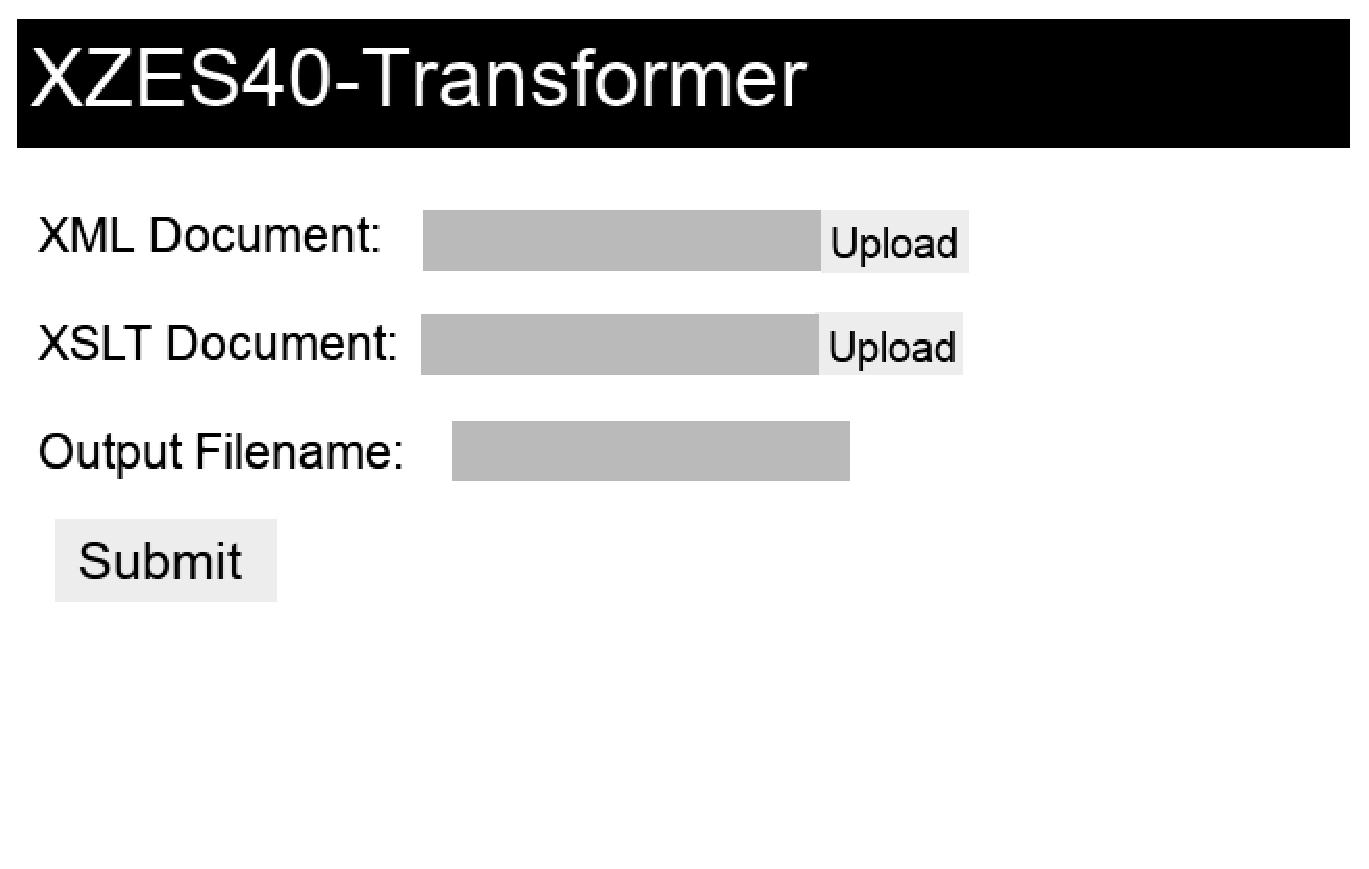
\includegraphics[width=0.5\textwidth]{figures/website-raw}
\end{figure}

\begin{figure}[h]
\centering
\caption{Diagram of dataflow}
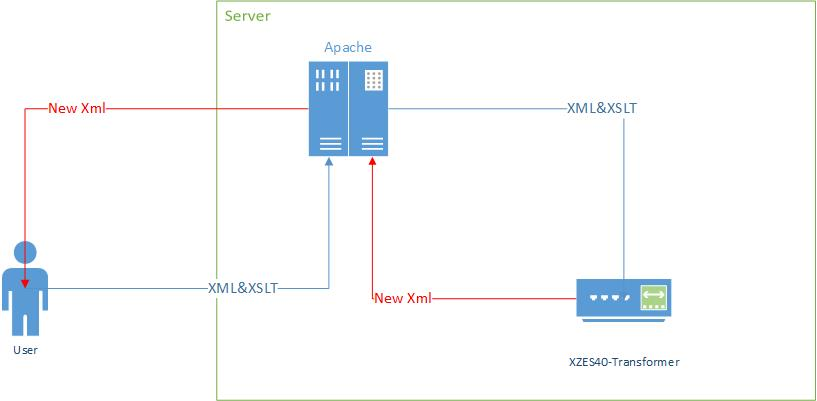
\includegraphics[width=0.5\textwidth]{figures/document-flow-digram}
\end{figure}

\begin{figure}[h]
\centering
\caption{Example use-cases of CLI interface}
\begin{lstlisting}
  Normal usage:
  $ xzes40cli --xml-file='./my-file.xml' --xslt-file='./my-other-file.xslt' --server='http://example.com/xzes40-transformer' --output-file='./newfile.xml' --port='8001'
  Sending XML and XSLT files to http:/example.com:8001/xzes40-transformer
  Transformation complete. Downloading response file to newfile.xml

  Sending a bad file:
  $ xzes40cli --xml-file='./badfile.jpg' --xslt-file='./badfile.txt' --server='http://example.com/xzes40-transformer'
  Sending XML and XSLT files to http:/example.com:80/xzes40-transformer
  ERROR: Server was unable to transform the requested files.

  Using inadequate parameters
  $ xzes40cli
  Please provide an xml file (--xml-file), xslt file (--xslt-file) and a host (--server).
\end{lstlisting}
\end{figure}


\clearpage
\namesigdate{Elijah C. Voigt}
\hfill
\namesigdate{Zixun Lu}
\hfill
\namesigdate{Shuai Peng}
\hfill
\namesigdate{Steven Hathaway}


\end{document}
